% Created 2023-08-19 Sat 22:28
% Intended LaTeX compiler: pdflatex
\documentclass[bigger]{beamer}
\usepackage[utf8]{inputenc}
\usepackage[T1]{fontenc}
\usepackage{graphicx}
\usepackage{longtable}
\usepackage{wrapfig}
\usepackage{rotating}
\usepackage[normalem]{ulem}
\usepackage{amsmath}
\usepackage{amssymb}
\usepackage{capt-of}
\usepackage{hyperref}
\usepackage{svg}
\usepackage{minted}
\usetheme[height=20pt]{Rochester}
\usecolortheme{dolphin}
\usefonttheme{}
\useinnertheme{}
\useoutertheme{}
\author{Vijay Paul Nayar}
\date{2023-08-29 Tue}
\title{OpenAPI and Service Integration}
\AtBeginSection[]{\begin{frame}<beamer>\frametitle{Presentat‌​‌​ion Agenda}\huge\secname\end{frame}}

\hypersetup{
 pdfauthor={Vijay Paul Nayar},
 pdftitle={OpenAPI and Service Integration},
 pdfkeywords={},
 pdfsubject={},
 pdfcreator={Emacs 29.1 (Org mode 9.6.7)}, 
 pdflang={English}}
\begin{document}

\maketitle
\begin{frame}{Outline}
\tableofcontents
\end{frame}


\begin{frame}[label={sec:org8fcd05a}]{Who am I?}
\begin{columns}
\begin{column}{0.4\columnwidth}
\begin{center}

\includegraphics[width=3cm]{PortraitLowRes.jpg}
\end{center}

Vijay Paul Nayar
\begin{itemize}
\item Java developer and CTO of a FinTech
\item Left CTO role to found own company
\end{itemize}
\end{column}

\begin{column}{0.6\columnwidth}
\begin{center}

\includegraphics[width=3cm]{funnel-icon.png}
\end{center}

\alert{Funnel-Labs.io}: Performant D apps.
\begin{itemize}
\item \alert{Funnel}: High performance data storage system for ride-hailing and micro-mobility companies.
\item \alert{Fiveum}: Office chat and video built to minimize interruptions and improve focus.
\end{itemize}
\end{column}
\end{columns}
\end{frame}

\begin{frame}[label={sec:org554819f}]{How did OpenAPI Come Up?}
\begin{columns}
\begin{column}{0.6\columnwidth}
\begin{itemize}
\item Built Funnel Service MVP\ldots{}
\begin{itemize}
\item How do customers pay for the service?
\begin{itemize}
\item Most services use credit-cards
\end{itemize}
\item How to easily add credit-card support?
\begin{itemize}
\item Stripe is popular and common
\end{itemize}
\item How to use Stripe?
\begin{itemize}
\item Stripe has a REST API, but it's huge
\end{itemize}
\item How do Java/Python do this?
\begin{itemize}
\item Generated OpenAPI client
\end{itemize}
\item Do such tools exist in D?
\begin{itemize}
\item \alert{No}, but they could.
\end{itemize}
\end{itemize}
\end{itemize}
\end{column}

\begin{column}{0.4\columnwidth}
\resizebox{\textwidth}{!}{
\begin{center}
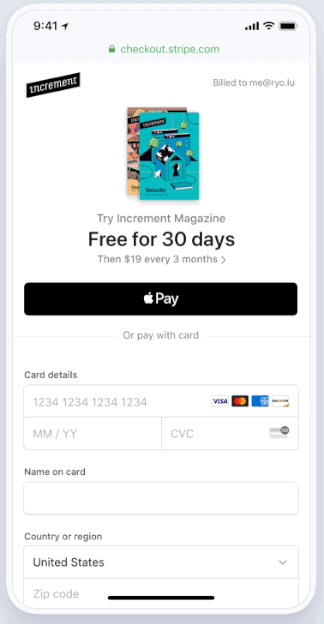
\includegraphics[width=1.2\linewidth]{StripeCheckout.png}
\end{center}
}
\end{column}
\end{columns}
\end{frame}

\section{Introduction}
\label{sec:orgb49fa3e}

\begin{frame}[label={sec:org701e58c}]{External Service Interoperability}
\begin{columns}
\begin{column}{0.6\columnwidth}
Companies often depend on useful external services.

For example:
\begin{itemize}
\item Stripe (financial transactions)
\item OpenAI (categorize sentiment, question/answer, content generation)
\item Slack (real-time communication)
\end{itemize}

Hand written clients are \alert{time-consuming} and \alert{error-prone}
\end{column}

\begin{column}{0.4\columnwidth}
\begin{center}
\includesvg[width=4cm]{Stripe_Logo_revised_2016}
\end{center}

\begin{center}
\includesvg[width=4cm]{OpenAI_Logo}
\end{center}

\begin{center}
\includesvg[width=4cm]{Slack_Technologies_Logo}
\end{center}
\end{column}
\end{columns}
\end{frame}

\begin{frame}[label={sec:org075ece3}]{Internal Service Interoperability}
Even internal services face interoperability challenges:
\begin{itemize}
\item Communication must be secure
\item Interfaces should be understandable and standardized
\item Multiple programming languages must be supported
(companies change technologies, different employees have different skills, etc.)
\end{itemize}

\begin{center}
\includesvg[height=2cm]{microservice-icon}
\end{center}
\end{frame}

\begin{frame}[label={sec:org12a0ffb}]{REST Interfaces}
(Re)presentational (S)tate (T)ransfer is an architectural style designed for the web
\begin{itemize}
\item Many forms, typically JSON/Avro/Protobuf over HTTPS
\item URLs arranged into "nouns" with HTTP Methods representing "verbs"
\item By itself, too vague to be uniform
\item Minor performance penalty for increased clarity
\end{itemize}

\begin{center}
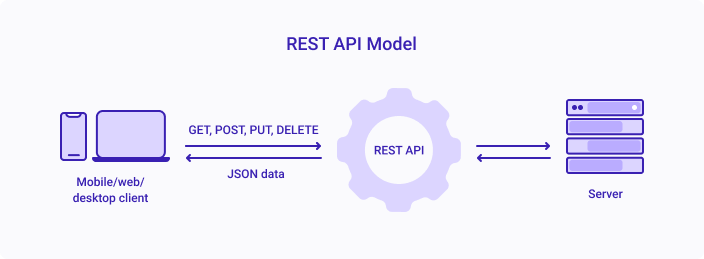
\includegraphics[width=12cm]{REST_API.png}
\end{center}
\end{frame}

\section{What is OpenAPI?}
\label{sec:org4c903cb}

\begin{frame}[label={sec:orgfbfe6ca}]{OpenAPI}
\begin{columns}
\begin{column}{0.25\columnwidth}
\begin{center}
\includesvg[width=3cm]{openapi-1}
\end{center}
\end{column}

\begin{column}{0.75\columnwidth}
\begin{itemize}
\item OpenAPI Specification is open standard to define HTTP APIs for external consumers
\begin{itemize}
\item Builds upon JSON Schemas \url{https://json-schema.org/}
\item Builds upon Swagger API description and documentation \url{https://swagger.io/}
\item Split from Swagger in 2016 to become the OpenAPI Initiative, a Linux Foundation project
\end{itemize}
\end{itemize}
\end{column}
\end{columns}
\end{frame}

\begin{frame}[label={sec:org3880b89}]{Benefits of OpenAPI Usage}
\begin{itemize}
\item Commonly used by major services, e.g. Stripe, Slack, OpenAI, and 2500+ more: \url{https://apis.guru/}
\item Standard formats mean tools can be used to generate client code with:
\begin{itemize}
\item request and responses
\item documentation
\item success and error codes
\end{itemize}
\item Creating an OpenAPI Specification enables low-effort cross-compatibility
\end{itemize}
\end{frame}

\begin{frame}[label={sec:org9c0fb32}]{}
\begin{center}
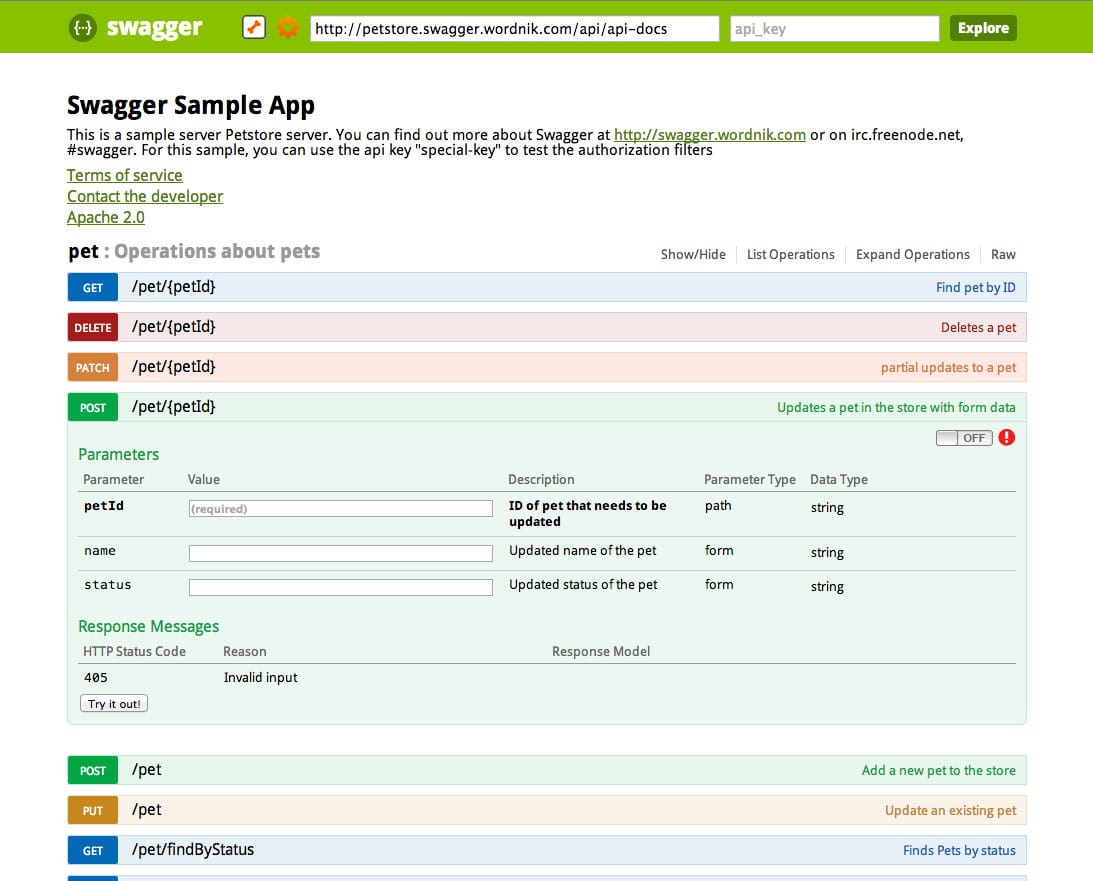
\includegraphics[width=1.2\linewidth]{swagger-ui.jpg}
\end{center}
\end{frame}

\begin{frame}[label={sec:org5268acc}]{Structure of an OpenAPI Specification}
\begin{itemize}
\item OpenAPI Specification is itself a JSON/YAML document
\end{itemize}

\begin{block}{OpenAPI Major Top-Level Attributes}
\scriptsize
\begin{center}
\begin{tabular}{lll}
\alert{Field Name} & \alert{Type} & \alert{Description}\\[0pt]
\hline
servers & [Server Object] & Connection info. for servers offering the API.\\[0pt]
paths & Paths Object & Method-specific actions by URL path.\\[0pt]
components & Components Object & Re-usable schemas for data by name.\\[0pt]
security & [Security Object] & Lists security mechanisms to access the API.\\[0pt]
\end{tabular}
\end{center}
\end{block}
\end{frame}

\begin{frame}[label={sec:orgf6cf7f3},fragile]{Defining API Endpoints - \#/paths}
 \begin{itemize}
\item Mapping from endpoint URL to details
\end{itemize}

\scriptsize
\begin{minted}[]{js}
{
  "paths": {
    "/files/{file_id}": {  // URL => Path Item
      "delete": {          // Method => Operation
        "operationId": "deleteFile",  // API-unique identifier
        "tags": [          // Tags for grouping documentation
          "OpenAI"
        ],
        "summary": "Delete a file.",  // A 1-liner for documentation.
        "parameters": [  // Request parameters in path/query/header/cookie
          {
            "in": "path",
            "name": "file_id",
            "required": true,
            "schema": {  // JSON Schema format is used.
              "type": "string"
            },
            "description": "The ID of the file to use for this request"
          }
        ],
        "responses": {  // Response data format by HTTP status
          "200": {
            "description": "OK",
            "content": {
              "application/json": {
                "schema": {
                  "$ref": "#/components/schemas/DeleteFileResponse"
                }
              }
            }
          }
        },
      },
      // All other methods: GET, POST, PUT, OPTIONS, HEAD
      "get": {
        ...
      }
    },
\end{minted}
\end{frame}

\begin{frame}[label={sec:org8368868}]{JSON Schemas}
\begin{itemize}
\item All data represented in JSON can be described using \href{https://datatracker.ietf.org/doc/html/draft-bhutton-json-schema-00}{JSON Schemas}.
\item Assertions are used to validate if data matches the schema:
\begin{description}
\item[{type}] Primitive valies like null, boolean, object, array, number, string
\item[{format}] How a type is used, e.g. date-time, email, uri, ipv4, etc.
\item[{enum}] Limit value to a predefined list.
\item[{allOf}] All validations must be satisfied.
\item[{anyOf}] One or more validation must be satisfied.
\item[{oneOf}] Exactly one validation must be satisfied.
\end{description}
\end{itemize}
\end{frame}

\begin{frame}[label={sec:org9f8fb88},fragile]{JSON Schema Example}
 \begin{columns}
\begin{column}{0.5\columnwidth}
An example schema:

\scriptsize
\begin{minted}[]{js}
{
  "components": {
    "schemas": {
      "CreateChatCompletionResponse": {
        "type": "object",
        "properties": {
          "id": {
            "type": "string"
          },
          "model": {
            "type": "string"
          },
          "choices": {
            "type": "array",
            "items": {
              "type": "object",
              "required": [
                "index",
                "message",
                "finish_reason"
              ],
              "properties": {
                ...
\end{minted}
\end{column}

\begin{column}{0.5\columnwidth}
An example instance complying with the schema:

\scriptsize
\begin{minted}[]{js}
{
  "id": "3d5e3472-3057-11ee-89d4-c3a0bb88b99f",
  "model": "gpt-3.5-turbo",
  "choices": [
    {
      "index": 3,
      "finish_reason": "length",
      "message": { ... }
    },
    ...
\end{minted}
\end{column}
\end{columns}
\end{frame}

\begin{frame}[label={sec:org1202539}]{Schema Primitive Types}
\begin{itemize}
\item Data Types:
\begin{itemize}
\item The "type" field corresponds broadly to a JSON type.
\item The "format" field clarifies details and usage.
\end{itemize}
\end{itemize}

\begin{center}
\begin{tabular}{lll}
\alert{type} & \alert{format} & \alert{Description}\\[0pt]
\hline
integer & int32 & signed 32 bits\\[0pt]
integer & int64 & signed 64 bits\\[0pt]
number & float & \\[0pt]
number & double & \\[0pt]
string & password & A hint to UIs to obscure input\\[0pt]
\end{tabular}
\end{center}
\end{frame}


\begin{frame}[label={sec:orgeb10ea8}]{Defining Common Components - \#/components}
APIs commonly have shared data types between paths.
\begin{itemize}
\item Error and Created responses
\item Query Parameters
\item Security headers
\end{itemize}

\resizebox{\textwidth}{!}{
\begin{center}
\begin{tabular}{lll}
 &  & \\[0pt]
\alert{Field Name} & \alert{Type} & \alert{Description}\\[0pt]
\hline
schemas & string => SchemaObj & Common schemas by name.\\[0pt]
responses & string => ResponseObj & Path responses, e.g. errors.\\[0pt]
parameters & string => ParameterObj & Request parameter types.\\[0pt]
requestBodies & string => RequestBodyObj & Request bodies for POST,PUT.\\[0pt]
headers & string => HeaderObj & Common data in HTTP headers.\\[0pt]
securitySchemes & string => SecuritySchemeObj & E.g. OAuth, Basic Auth, etc.\\[0pt]
\end{tabular}
\end{center}
}
\end{frame}

\begin{frame}[label={sec:orgdc070d1},fragile]{Reusing Components}
 \begin{itemize}
\item Once defined, components can be referenced by their location in the OpenAPI Schema.
\item Substitute type definition with a "\$ref" to a component.
\end{itemize}

\begin{minted}[]{js}
"properties": {
  "index": {
    "type": "integer"
  },
  "message": {
    "$ref": "#/components/schemas/ChatCompletionResponseMessage"
  },
\end{minted}
\end{frame}

\section{Managing OpenAPI Specs}
\label{sec:org9c81e22}

\begin{frame}[label={sec:org8fc2b23}]{Creating OpenAPI Specifications}
\begin{itemize}
\item D currently lacks tools to extract specification from code.
\item Open question whether it is better to:
\begin{itemize}
\item Generate specification from code
\begin{itemize}
\item Easier to keep specification up to date
\item Language/Framework-specific projects like \href{https://springdoc.org/}{SpringDoc}
\end{itemize}
\item Generate interfaces from specification
\begin{itemize}
\item Easier tool integration and multi-language support
\item Projects like \href{https://github.com/OpenAPITools/openapi-generator}{openapi-generator}
\end{itemize}
\end{itemize}
\end{itemize}
\end{frame}

\begin{frame}[label={sec:orge94403f}]{OpenAPI Specification from Code}
\begin{itemize}
\item Systems like SpringDoc are specific to language (Java) and web framework (Spring)
\item OpenAPI Specification is updated with code changes
\end{itemize}

\begin{center}
\includesvg[height=5cm]{spec}
\end{center}
\end{frame}

\begin{frame}[label={sec:orgfd7523f}]{OpenAPI Specification from Code}
\begin{itemize}
\item What happens when a service is split?
\item What if multiple technologies are used?
\end{itemize}

\begin{center}
\includesvg[height=5cm]{spec2}
\end{center}
\end{frame}

\begin{frame}[label={sec:orge3042c3}]{Code from OpenAPI Specification}
\begin{itemize}
\item Requires clients/servers to regenerate code after changes
\end{itemize}

\begin{center}
\includesvg[height=5cm]{spec3}
\end{center}
\end{frame}

\begin{frame}[label={sec:org1d7c439},fragile,shrink=30]{Java SpringDoc OpenAPI Annotations}
 \begin{minted}[]{java}
@SecurityScheme(name = "petstore_auth", type = SecuritySchemeType.OAUTH2, flows = @OAuthFlows(implicit = @OAuthFlow(authorizationUrl = "https://petstore3.swagger.io/oauth/authorize", scopes = {
                @OAuthScope(name = "write:pets", description = "modify pets in your account"),
                @OAuthScope(name = "read:pets", description = "read your pets") })))
@Tag(name = "pet", description = "the pet API")
public interface PetApi {
        @Operation(summary = "Add a new pet to the store",
            description = "Add a new pet to the store",
            security = { @SecurityRequirement(name = "petstore_auth", scopes = { "write:pets", "read:pets" }) },
            tags = { "pet" })
        @ApiResponses(value = {
            @ApiResponse(responseCode = "200",
                description = "Successful operation",
                content = {
                  @Content(mediaType = "application/xml", schema = @Schema(implementation = Pet.class)),
                  @Content(mediaType = "application/json", schema = @Schema(implementation = Pet.class)) }),
            @ApiResponse(responseCode = "405", description = "Invalid input")
        })
        @PostMapping(value = "/pet", consumes = { "application/json", "application/xml", "application/x-www-form-urlencoded" })
        default void addPet(
            @Parameter(description = "Create a new pet in the store", required = true) @Valid @RequestBody Pet pet) {
          // return getDelegate().addPet(pet);
        }

\end{minted}
\end{frame}

\section{Useful D Features}
\label{sec:org522b973}

\begin{frame}[label={sec:org3dc95d7},fragile]{Mixins}
 The \texttt{mixin} expression takes a list of \texttt{string} arguments representing a complete D statement and
turns them into code.
\begin{itemize}
\item Can make use of variables known at compile-time, e.g. those provided by templates
\item Useful for code that declares variables or methods with parameterized identifiers
\end{itemize}

\begin{minted}[]{d}
mixin("private bool _myValue;");

string N = "yourVal";
mixin("private bool", "_", N, ";");
\end{minted}
\end{frame}

\begin{frame}[label={sec:orgd1bfaed},fragile]{Mixin Templates}
 A \texttt{mixin template} encloses declarations of fields, functions, classes, structs, etc. When referenced
in code with compile-time parameters, it inserts those declarations in the scope in which it was
called.
\begin{itemize}
\item \alert{Mixin Templates}: Re-useable code generation
\end{itemize}

\begin{columns}
\begin{column}{0.6\columnwidth}
\scriptsize
\begin{minted}[]{d}
import std.traits : isAssignable;
import std.string : capitalize;
import std.typecons : Nullable;

mixin template AddField(C, T, string N) {
  // Declare the variable.
  mixin(T, " ", N, ";");
  mixin(  // Define  setter function.
      C, " set", capitalize(N), "(ST)(ST val) ",
      "if (isAssignable!(T, ST)) {",
      "  this.", N, " = val;",
      "  return this;",
      "}");
}
\end{minted}
\end{column}

\begin{column}{0.4\columnwidth}
\scriptsize
\begin{minted}[]{d}
// Example usage
class Fish {
  mixin AddField!(typeof(this),
      Nullable!int, "age");
  mixin AddField!(typeof(this),
      Nullable!string, "job");
}

unittest {
  import std.stdio;
  Fish f = new Fish()
      .setAge(42)
      .setJob("Accountant");
  writeln(f.age, " ", f.job);
}
\end{minted}
\end{column}
\end{columns}
\end{frame}

\begin{frame}[label={sec:orgc8a5a55},fragile]{Static ForEach}
 \texttt{static foreach} statements generate repeated lines of code in the same scope in which they occur.
\begin{itemize}
\item \alert{static foreach}: Loop over compile-time data, such as class members.
\end{itemize}

\begin{columns}
\begin{column}{0.6\columnwidth}
\scriptsize
\begin{minted}[]{d}
import std.traits : Fields, FieldNameTuple,
                    BaseClassesTuple;
// Add setters for a single class.
mixin template AddClassSetters(C) {
  static foreach (
      size_t i; iota(Fields!(C).length)) {
    mixin AddSetter!(
        Fields!(C)[i], FieldNameTuple!(C)[i]);
  }
}
// Add setters for full class hierarchy.
mixin template AddSetters(C) {
  static foreach (B; BaseClassesTuple!(C)) {
    mixin AddSetters!(B);
  }
  mixin AddClassSetters!(C);
}
\end{minted}
\end{column}

\begin{column}{0.4\columnwidth}
\scriptsize
\begin{minted}[]{d}
class A {
  int a1;
  string a2;
}

class B : A {
  float b1;
  mixin AddSetters!(typeof(this));
}

unittest {
  import std.stdio;
  B b = new B()
    .setA1(3)
    .setA2("ham")
    .setB1(2.9);
}
\end{minted}
\end{column}
\end{columns}
\end{frame}

\section{D Project: openapi-client}
\label{sec:org3282a23}

\begin{frame}[label={sec:org8b6073b}]{Simple OpenAPI Client in D}
\href{https://code.dlang.org/}{code.dlang.org} project: \href{https://code.dlang.org/packages/openapi-client}{openapi-client}
\begin{itemize}
\item Consistent interface created/updated in seconds
\item Creates data types from OpenAPI Specification
\item Creates client to call endpoints
\item Configurable server and security controls
\end{itemize}

\begin{center}
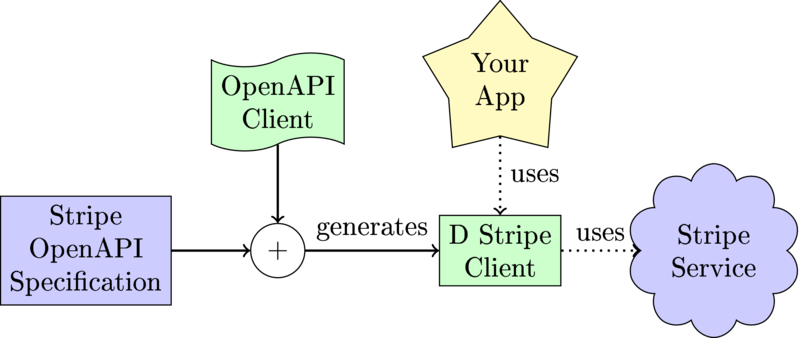
\includegraphics[width=0.9\textwidth]{openapi-client-flow.png}
\end{center}
\end{frame}

\begin{frame}[label={sec:org57a2626},fragile]{openai-client: Creating an OpenAI Client}
 \begin{enumerate}
\item Download the OpenAPI Specification from GitHub:
\begin{verbatim}
curl https://raw.githubusercontent.com/openai/
  openai-openapi/master/openapi.yaml
  -o openapi.yaml
\end{verbatim}
\item Convert to JSON format:
\begin{verbatim}
yq openapi.yaml -o json > openapi.json
\end{verbatim}
\item Invoke \texttt{openapi-client} to generate code:
\begin{verbatim}
dub run openapi-client@2.0.1 --
  --openApiSpec=json/openapi.json
  --packageRoot=openai
\end{verbatim}
\item Done!
\end{enumerate}
\end{frame}

\begin{frame}[label={sec:orge2f41fb},fragile]{openai-client: Generated Models}
 \begin{minted}[]{d}
// File: openapi/model/CreateImageEditRequest.d
class CreateImageEditRequest {
  /**
   * The number of images to generate. Must be between 1 and 10.
   */
  @vibeName("n")
  @vibeOptional
  @vibeEmbedNullable
  Nullable!(int) n;

  /**
   * The image to edit. Must be a valid PNG file, less than 4MB, and square. If mask is not
   * provided, image must have transparency, which will be used as the mask.
   */
  @vibeName("image")
  @vibeOptional
  string image;

  // ...
\end{minted}
\end{frame}

\begin{frame}[label={sec:org36c5527},fragile]{openai-client: Generated Models}
 \begin{itemize}
\item Optional fields are \texttt{Nullable}.
\item Nested objects as static inner classes
\item Documentation included
\item Builder pattern used to ease object creation
\end{itemize}
\end{frame}

\begin{frame}[label={sec:org1eddb2e},fragile]{openai-client: Generated Services}
 \begin{minted}[]{d}
// File: openai/service/image_edits_service.d
/**
 * Service to make REST API calls to paths beginning with: /images/edits
 */
class ImagesEditsService {
  /**
   * Creates an edited or extended image given an original image and a prompt.
   * See_Also: HTTP POST `/images/edits`
   */
  void createImageEdit(
      CreateImageEditRequest requestBody,
      CreateImageEditResponseHandler responseHandler,
      ) {
    ApiRequest requestor = new ApiRequest(
        HTTPMethod.POST,
        Servers.getServerUrl(),
        "/images/edits");
    requestor.setHeaderParam("Content-Type", "multipart/form-data");
    Security.apply(requestor);
    requestor.makeRequest(requestBody, responseHandler);
  }
\end{minted}
\end{frame}

\begin{frame}[label={sec:org7faa1be},fragile,shrink=15]{openai-client: Using Services}
 \begin{minted}[]{d}
// Service classes group API functionality by path, e.g. /completions
auto service = new CompletionsService();
// Invoke an API endpoint, this one is for POST /completions
service.createCompletion(
    // Define the request body with a builder.
    CreateCompletionRequest.builder()
        .model("text-davinci-003")
        .prompt(Json("What is the cutest breed of rabbit? "))
        .echo(true)
        .maxTokens(2048)
        .build(),
    // ResponseHandlers have an attribute for each valid response.
    CompletionsService.CreateCompletionResponseHandler.builder()
        .handleResponse200((CreateCompletionResponse response) {
          logDebug("%s", serializeToJson(response).toString());
        })
        .build());
\end{minted}
\end{frame}

\begin{frame}[label={sec:orgff13409},fragile]{openai-client: Server Response}
 \begin{minted}[]{js}
{
  "object": "text_completion",
  "created": 1690899388,
  "usage": {
    "prompt_tokens": 10,
    "total_tokens": 68,
    "completion_tokens": 58
  },
  "id": "cmpl-7ikSiD1IqwHn4XMwg8K04lvx2DnL9",
  "model": "text-davinci-003",
  "choices": [
    {
      "index": 0,
      "text": "What is the cutest breed of rabbit?

               The debate for which rabbit breed is the cutest is subjective,
               as it will depend on what the individual finds appealing. Some
               popular breeds that are known for their cute looks include the
               Holland Lop, Mini Rex, Jersey Wooly, Mini Lop, and Netherland Dwarf.",
      "logprobs": null,
      "finish_reason": "stop"
    }
  ]
}
\end{minted}
\end{frame}

\begin{frame}[label={sec:org37a7e42}]{Future Plans}
\begin{columns}
\begin{column}{0.5\columnwidth}
\begin{itemize}
\item Move spec-first efforts to more mature projects like \href{https://github.com/OpenAPITools/openapi-generator}{openapi-generator}
\begin{itemize}
\item Add D client and server-stub \href{https://github.com/OpenAPITools/openapi-generator/wiki/How-to-add-a-generator-for-a-new-language-or-framework}{generators}
\end{itemize}
\item Consider code-first integration via annotations in frameworks like \href{https://vibed.org/}{Vibe.d}
\end{itemize}
\end{column}

\begin{column}{0.5\columnwidth}
\resizebox{\textwidth}{!}{
\begin{center}
\includesvg[width=1.2\linewidth]{openapi-generator-logo}
\end{center}
}
\end{column}
\end{columns}
\end{frame}

\begin{frame}[label={sec:org3485a40}]{Thank You}
Thank you for your interest and attention!
\end{frame}
\end{document}